\documentclass{beamer}
\let\vec\mathbf
\mode<presentation>
\usepackage{amsmath}
\usepackage{amssymb}
%\usepackage{advdate}
\usepackage{adjustbox}
%\usepackage{subcaption}
\usepackage{enumitem}
\usepackage{multicol}
\usepackage{mathtools}
\usepackage{listings}
\usepackage{url}
\usetheme{Boadilla}
\usecolortheme{lily}
\setbeamertemplate{footline}
{
  \leavevmode%
  \hbox{%
  \begin{beamercolorbox}[wd=\paperwidth,ht=2.25ex,dp=1ex,right]{author in head/foot}%
    \insertframenumber{} / \inserttotalframenumber\hspace*{2ex} 
  \end{beamercolorbox}}%
  \vskip0pt%
}
\setbeamertemplate{navigation symbols}{}
\providecommand{\nCr}[2]{\,^{#1}C_{#2}} % nCr
\providecommand{\nPr}[2]{\,^{#1}P_{#2}} % nPr
\providecommand{\mbf}{\mathbf}
\providecommand{\pr}[1]{\ensuremath{\Pr\left(#1\right)}}
\providecommand{\qfunc}[1]{\ensuremath{Q\left(#1\right)}}
\providecommand{\sbrak}[1]{\ensuremath{{}\left[#1\right]}}
\providecommand{\lsbrak}[1]{\ensuremath{{}\left[#1\right.}}
\providecommand{\rsbrak}[1]{\ensuremath{{}\left.#1\right]}}
\providecommand{\brak}[1]{\ensuremath{\left(#1\right)}}
\providecommand{\lbrak}[1]{\ensuremath{\left(#1\right.}}
\providecommand{\rbrak}[1]{\ensuremath{\left.#1\right)}}
\providecommand{\cbrak}[1]{\ensuremath{\left\{#1\right\}}}
\providecommand{\lcbrak}[1]{\ensuremath{\left\{#1\right.}}
\providecommand{\rcbrak}[1]{\ensuremath{\left.#1\right\}}}
\theoremstyle{remark}
\newtheorem{rem}{Remark}
\newcommand{\sgn}{\mathop{\mathrm{sgn}}}

\providecommand{\res}[1]{\Res\displaylimits_{#1}} 
\providecommand{\norm}[1]{\lVert#1\rVert}
\providecommand{\mtx}[1]{\mathbf{#1}}

\providecommand{\fourier}{\overset{\mathcal{F}}{ \rightleftharpoons}}
%\providecommand{\hilbert}{\overset{\mathcal{H}}{ \rightleftharpoons}}
\providecommand{\system}{\overset{\mathcal{H}}{ \longleftrightarrow}}
 %\newcommand{\solution}[2]{\textbf{Solution:}{#1}}
%\newcommand{\solution}{\noindent \textbf{Solution: }}
\providecommand{\dec}[2]{\ensuremath{\overset{#1}{\underset{#2}{\gtrless}}}}
\newcommand{\myvec}[1]{\ensuremath{\begin{pmatrix}#1\end{pmatrix}}}

\title{Matrices in Geometry - 9.4.48}
\author{EE25BTECH11035 Kushal B N}
\date{}

\begin{document}

\maketitle

\section{Problem Statement}
\begin{frame}
\frametitle{Problem Statement}
Find two consecutive odd positive integers sum of whose squares is 290.
\end{frame}

\section{Solution}
\begin{frame}{Solution}
Let the two consecutive odd positive integers be $n$ and $(n+2)$, so that we get,
\begin{equation}
    n^2 + (n+2)^2 = 290
\end{equation}

\begin{equation}
    \implies 2n^2 + 2n - 143 = 0
\end{equation}
Representing this equation as a conic section
\begin{equation}
    \vec{x}^{\top}\vec{V}\vec{x} + 2\vec{u}^{\top}\vec{x} + f = 0, \vec{V} = \myvec{1&0\\0&0}, \vec{u} = \myvec{1\\-1/2}, f = -143
\end{equation}
We need to find intersection points with $y = 0$, that is, the X-axis.
\begin{equation}
    \vec{x} = \vec{h} + k\vec{m}, \vec{h} = \myvec{0\\0}, \vec{m} = \myvec{1\\0}
\end{equation}
\end{frame}

\begin{frame}{Solution}
Substituting $\vec{x} = k\vec{m}$

\begin{equation}
    k^2\vec{m}^{\top}\vec{V}\vec{m} + 2k\vec{u}^{\top}\vec{m} + f = 0
\end{equation}

\begin{equation}
    \implies k = \frac{1}{2}\sbrak{-2\vec{u}^{\top}\vec{m} \pm \sqrt{4(\vec{u}^{\top}\vec{m})^2 - 4f\vec{m}^{\top}\vec{V}\vec{m}}}
\end{equation}

\begin{equation}
    \implies k = -\vec{u}^{\top}\vec{m} \pm \sqrt{(\vec{u}^{\top}m)^2 - f\vec{m}^{\top}\vec{V}\vec{m}}
\end{equation}

\begin{equation}
    \vec{u}^{\top}\vec{m} = \myvec{1 & -1/2}\myvec{1\\0} = 1
\end{equation}

\begin{equation}
    \vec{m}^{\top}\vec{V}\vec{m} = \myvec{1&0}\myvec{1&0\\0&0}\myvec{1\\0} = 1
\end{equation}

\begin{equation}
    k = -1 \pm \sqrt{(1)^2 - (-143)(1)}
\end{equation}
\end{frame}

\begin{frame}{Solution}
\begin{equation}
    k = -1 \pm \sqrt{144}
\end{equation}

\begin{equation}
    \implies k = -1 \pm 12 \implies \fbox{$k = 11 \text{ OR } k = -13$}
\end{equation}

Substituing $k$ into $\vec{x}$, we get
\begin{equation}
    \vec{x} = \myvec{11\\0} \text{ OR } \vec{x} = \myvec{-13\\0}
\end{equation}
This implies that the roots of the equation are 11 and -13.
So, we have
\begin{equation}
    \implies \fbox{$n = 11$}
\end{equation}
\end{frame}

\section{Final Answer}
\begin{frame}{Final Answer}
$\therefore$ The two consecutive odd positive integers whose sum of squares is 290 are 13 and 11.

\begin{figure}[H]
    \centering
    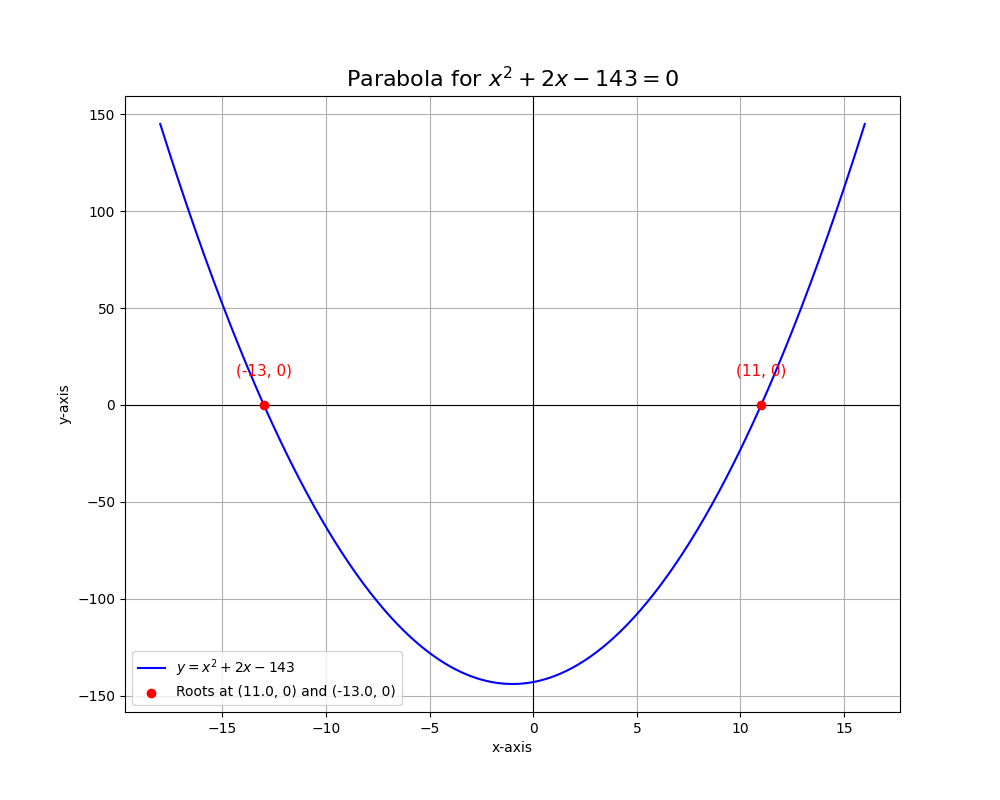
\includegraphics[width=0.55\columnwidth]{figs/1.png}
    \caption{Plot for 9.4.48}
\end{figure}
\end{frame}

\end{document}